\documentclass[a4paper,12pt]{article}
\usepackage{tabularx}
\usepackage{amsmath}
\usepackage[utf8]{inputenc}
\usepackage{multicol}
\usepackage{amsmath, amssymb, amsthm}
\usepackage{graphicx}
\usepackage{enumitem}
\usepackage{array}
\usepackage[left=2cm, right=2cm, top=2cm, bottom=2cm]{geometry}
\usepackage{fancyhdr}
\usepackage{xfp}
\usepackage{pgf}
\usepackage{tikz}

\usepackage{graphicx}
\usepackage{fancyhdr}
\setlength{\headheight}{28pt} % genug Platz für das Logo
\pagestyle{fancy}
\fancyhf{} % alles leeren
\fancyhead[L]{\includegraphics[height=1.2cm]{logo.png}}
\fancyhead[C]{\small Klassenarbeit – Funktionale Zusammenhänge\\ Potenzfunktionen \ (Kl. G9A)}
\fancyhead[R]{\small Name:\ \rule{2.8cm}{0.4pt}}
\fancyfoot[C]{\thepage}

\fancyfoot[C]{Seite \thepage \enspace\textbullet\enspace J.\,Mycan \textcopyright~2025}

\renewcommand{\footrulewidth}{0.4pt}




%\pagestyle{fancy}
%\lhead{Klassenarbeit 45min.}
%\chead{Heinrich-von-Kleist-Schule}
%\rhead{Mathematik - G8A}
%\lfoot{}
%\cfoot{Seite \thepage}
%\rfoot{}

\newcommand{\punkteA}{6}
\newcommand{\punkteB}{6}
\newcommand{\punkteC}{6}
\newcommand{\punkteD}{18}
\newcommand{\punkteE}{6}
%\newcommand{\punkteF}{12}

\newcommand{\maxSumme}{42}
\newcommand{\noteEinsMin}{\fpeval{round(\maxSumme * 0.95,0)}}
\newcommand{\noteZweiMin}{\fpeval{round(\maxSumme * 0.80,0)}}
\newcommand{\noteDreiMin}{\fpeval{round(\maxSumme * 0.60,0)}}
\newcommand{\noteVierMin}{\fpeval{round(\maxSumme * 0.45,0)}}
\newcommand{\noteFunfMin}{\fpeval{round(\maxSumme * 0.20,0)}}
\newcommand{\noteSechsMin}{0}

\newcommand{\summe}{%
	\pgfmathparse{\punkteA + \punkteB + \punkteC + \punkteD + \punkteE}%
	\pgfmathprintnumber{\pgfmathresult}}

\begin{document}
	
%	\begin{center}
%		\textbf{Klassenarbeit - Lineare Funktionen und LGS}
%	\end{center}
	
%	\textbf{Vor- und Nachname:} \underline{\hspace{10cm}}\\[0.1cm]
	Die Lösungen sowie Lösungswege sollten klar strukturiert und gut nachvollziehbar sein.\\[0.1cm]
	

	
	
	% -------------------------------------------------
	% Aufgabe 1
	% -------------------------------------------------
	\textbf{Aufgabe 1 ( Punkte)}\\
\textbf{Aufgabe: Zuordnung von Parabeln}\\[0.5em]
Im Koordinatensystem sind vier verschiedene Parabeln eingezeichnet:
zwei nach oben geöffnet, zwei nach unten geöffnet.
Ordne jedem Graphen (I–IV) eine passende Funktionsgleichung zu.
Eine der fünf Funktionsgleichungen passt zu keinem der Graphen.

\begin{center}
	\begin{tikzpicture}[scale=0.9]
		% Koordinatensystem [-5,5] x [-5,5] mit Gitter
		\draw[step=1,very thin,gray!40] (-5,-5) grid (5,5);
		\draw[->] (-5,0) -- (5.5,0) node[below right] {$x$};
		\draw[->] (0,-5) -- (0,5.5) node[above] {$y$};
		
		% Achsenbeschriftung (einige Ticks)
		\foreach \x in {-4,-2,2,4}
		\draw (\x,0.1) -- (\x,-0.1) node[below=2pt] {\small \x};
		\foreach \y in {-4,-2,2,4}
		\draw (0.1,\y) -- (-0.1,\y) node[left=2pt] {\small \y};
		
		% Parabel I: f(x) = 1/4 x^2 - 2  (nach oben geöffnet, Scheitel bei (0|-2))
		\draw[thick,domain=-4.5:4.5,smooth,variable=\x]
		plot ({\x},{0.25*\x*\x - 2});
		\node[below right] at (0,-2) {\small I};
		
		% Parabel II: f(x) = 1/4 (x-2)^2 + 1  (nach oben geöffnet, Scheitel bei (2|1))
		\draw[thick,dashed,domain=-1:5,smooth,variable=\x]
		plot ({\x},{0.25*(\x-2)*(\x-2) + 1});
		\node[above right] at (2,1) {\small II};
		
		% Parabel III: f(x) = -1/4 x^2 + 3  (nach unten geöffnet, Scheitel bei (0|3))
		\draw[thick,dotted,domain=-4:4,smooth,variable=\x]
		plot ({\x},{-0.25*\x*\x + 3});
		\node[above right] at (0,3) {\small III};
		
		% Parabel IV: f(x) = -1/2 (x+3)^2 + 1  (nach unten geöffnet, Scheitel bei (-3|1))
		\draw[thick,loosely dashed,domain=-5:1,smooth,variable=\x]
		plot ({\x},{-0.5*(\x+3)*(\x+3) + 1});
		\node[above left] at (-3,1) {\small IV};
		
	\end{tikzpicture}
\end{center}

\noindent
\textbf{Zuordnungsaufgabe:}\\
Ordne jedem Graphen I–IV genau eine Funktionsgleichung zu.
Eine Funktionsgleichung bleibt übrig.

\begin{itemize}
	\item[A)] \(f(x) = \dfrac{1}{4}x^{2} - 2\)
	\item[B)] \(f(x) = \dfrac{1}{4}(x-2)^{2} + 1\)
	\item[C)] \(f(x) = -\dfrac{1}{4}x^{2} + 3\)
	\item[D)] \(f(x) = -\dfrac{1}{2}(x+3)^{2} + 1\)
	\item[E)] \(f(x) = \dfrac{1}{2}x^{2}\)
\end{itemize}



	
	% -------------------------------------------------
	% Aufgabe 2
	% -------------------------------------------------
	\textbf{Aufgabe 2 ( Punkte)}\\
Die Flugkurve eines Speers entspricht der abgebildeten Parabel und kann durch folgende
quadratische Funktion beschrieben werden:
\[
f(x) = -0,0125 \cdot x^{2} + 0{,}5 \cdot x + 2{,}2.
\]
Dabei werden \(f(x)\) und \(x\) jeweils in Metern gemessen.

\begin{enumerate}
	\item[a)] Ermittle die Abwurfhöhe des Speers.
	\item[b)] Berechne, in welcher horizontalen Entfernung vom Abwurf der Speer gelandet ist.
	\item[c)] Berechne die maximale Flughöhe des Speers.
\end{enumerate}
	
	% -------------------------------------------------
	% Aufgabe 3
	% -------------------------------------------------
	\textbf{Aufgabe 3 ( Punkte)}\\
	Ein Rechteck soll so konstruiert werden, dass seine Breite \(x\) Meter beträgt und seine Länge
	durch die Funktion
	\[
	L(x) = 12 - x
	\]
	gegeben ist. Die Fläche des Rechtecks ergibt sich damit durch
	\[
	A(x) = x \cdot L(x).
	\]
	
	\begin{enumerate}
		\item Stelle die Flächenfunktion \(A(x)\) explizit als quadratische Funktion auf.
		\item Bestimme durch geeignete Verfahren den Wert von \(x\), bei dem die Fläche maximal wird.
		\item Berechne die maximale Fläche.
	\end{enumerate}
	\vspace{1 cm}
	%\newpage
	% -------------------------------------------------
	% Aufgabe 4
	% -------------------------------------------------
	\textbf{Aufgabe 4 ( Punkte)}\\
	Gegeben sind die Funktionen
	\[
	f(x) = 5x^6 - 3x^2 - 4
	\]
	und
	\[
	g(x) = 2x^5+ 3x^3 - 3x.
	\]
	
	\begin{enumerate}
		\item[(a)] Untersuche die Graphen von \(f\) und \(g\) auf Symmetrie.
		\begin{itemize}
			\item Entscheide für jede der beiden Funktionen, ob ihr Graph \textbf{achsensymmetrisch zur \(y\)-Achse}, \textbf{punktsymmetrisch zum Ursprung} oder \textbf{keine der beiden Symmetrien} besitzt.
			\item Begründe deine Entscheidung jeweils mit einem passenden Merkmal der Funktionsgleichung oder mit einer Skizze.
		\end{itemize}
		
		\item[(b)] Beweise deine Vermutungen aus Teilaufgabe (a) rechnerisch:

	\end{enumerate}
	
	% -------------------------------------------------
	% Aufgabe 5
	% -------------------------------------------------
	\textbf{Aufgabe 5 ( Punkte)}\\
	Löse die folgenden quadratischen Gleichungen. Begründe jeden Schritt kurz (z.\,B. quadratische Ergänzung, Mitternachtsformel, Ausklammern).
	
	\begin{enumerate}
		\item[(a)] 
		\[
		x^2 - 6x + 5 = 0
		\]
		Löse die Gleichung und gib beide Lösungen an.
		
		\item[(b)]
		\[
		3x^2 + 12x = 9
		\]
		Bringe die Gleichung zunächst auf eine Seite und löse sie anschließend mit einem Verfahren deiner Wahl.
		
		\item[(c)] 
		\[
		(x - 4)(x + 2) = 10
		\]
		Multipliziere aus, forme eine quadratische Gleichung und löse sie.
		
		\item[(d)] Zusatz (optional):  
		Prüfe für jede Gleichung, ob die Lösungen reell sind oder ob keine reellen Lösungen existieren.
	\end{enumerate}

	% -------------------------------------------------
	% Aufgabe 6
	% -------------------------------------------------
	\textbf{Aufgabe 6 ( Punkte)}\\
	Gegeben ist eine quadratische Funktion, deren Nullstellen bei
	\[
	x_1 = -2 \quad \text{und} \quad x_2 = 4
	\]
	liegen. Außerdem verläuft der Graph der Funktion durch den Punkt
	\[
	P(1 \mid -9).
	\]
	
	\begin{enumerate}
		\item Bestimme den Funktionsterm der quadratischen Funktion in der in der normal Form.
		
		\item Gib anschließend die Funktionsgleichung in der Produktform

		an und überprüfe, ob sie mit deinem Ergebnis aus Teil (1) übereinstimmt.
	\end{enumerate}
	\vspace{6cm}

	
	\vspace{2cm}
	\textbf{Kenntnisnahme eines Elternteils:} \hrulefill \hfill \textbf{Note:} \hrulefill
	
\end{document}
